%%% mode: latex
%%% TeX-master: t
%%% End:

\chapter{面向临床诊疗链的多智能体协作系统构建与威胁建模}
\label{cha:methodology}

\section{临床SOP流程的形式化建模}
\label{sec:sop_modeling}

\subsection{临床诊疗链的抽象}
\label{subsec:clinical_chain}

医疗诊疗活动本质上是一个遵循标准作业程序（Standard Operating Procedure, SOP）的链式决策过程。从患者初诊到最终治疗方案的确立，临床需依次完成病史采集、辅助检查、诊断推理和处方制定等关联步骤。本文将这一连续的诊疗过程抽象为一个由状态节点构成的拓扑链，形式化表示为 $S_1(\text{问诊}) \to S_2(\text{检查}) \to S_3(\text{诊断}) \to S_4(\text{处方})$。其中，每个节点对应诊疗流程中的一个关键环节，节点间的有向边代表信息的传递与依赖关系。

当引入多智能体技术辅助诊疗时，不同环节可由具备相应专长的智能体分别承担。这种分工协作模式虽然提升了单点任务的处理能力，但也打破了传统人工诊疗的一体化决策过程，客观上引入了跨模块信息的传递风险\cite{alami2025multi,medguards2025}。

需要强调的是，医疗领域的人工智能系统与通用领域智能体存在本质区别。通用智能体系统通常采用自由规划（Free Planning）策略，允许智能体根据任务目标自主决策执行路径。而在医疗场景中，智能体必须严格遵循既定的临床SOP约束，不能随意跳过或重排诊疗步骤。世界卫生组织发布的临床诊疗指南\cite{who2021clinical}以及中国卫生健康委员会制定的《临床诊疗规范》\cite{nhc2020clinical}均明确要求诊疗活动应遵循标准化流程，确保各环节有序衔接。例如，在未完成必要检查之前直接开具处方是严重的医疗违规行为，智能体系统必须在架构层面防止此类情况的发生。

基于上述分析，本文构建的临床诊疗链抽象具备三个核心特征：其一，线性推进。诊疗步骤按既定顺序执行，下游输出严格依赖上游输入；其二，职责分离。各状态节点由专门化智能体负责；其三，边界约束。智能体的行动不可超出其对应环节的职权范围。这一模型为后续开展多智能体的安全性评估奠定了理论基础，也为分析级联错误提供了结构化框架。

需要指出的是，真实的临床诊疗过程通常包含多轮交互与反馈。例如，医生可能根据初步检查的结果，向患者补充询问病史。然而，本文在系统建模与安全评估时将其抽象为单向的线性信息流模型，主要基于以下两点客观限制与考量：

其一，受限于真实医疗数据的静态特征。本研究采用真实的既往临床病历作为评估依据。在测试过程中，如果智能体提出进行数据集中未包含的检查项目，系统无法在现实中动态补充该检查结果。因此，为了保证自动化评估能够顺利闭环，必须将智能体的交互流程限制为严格遵循数据集中已有的单向诊疗顺序。

其二，多轮交互过程在时间轴上可展开为单向序列。虽然实际诊疗会发生环节上的回环，但在记录和分析信息传递时，可以将其按时间顺序展开。例如，将“问诊与检查的反复”表示为“首次问诊 $\to$ 初步检查 $\to$ 补充问诊”的单向序列。在这一序列中，即便同一类型的诊疗环节再次出现，也被视为时间轴上的一个新节点。这种展开方式不仅准确保留了真实的信息流向，还有利于后续清晰地追踪并计算错误信息在各步骤间的传递情况。

图\ref{fig:clinical_abstraction}展示了从真实临床流程到多智能体映射的抽象过程。

\begin{figure}[!htbp]
    \centering
    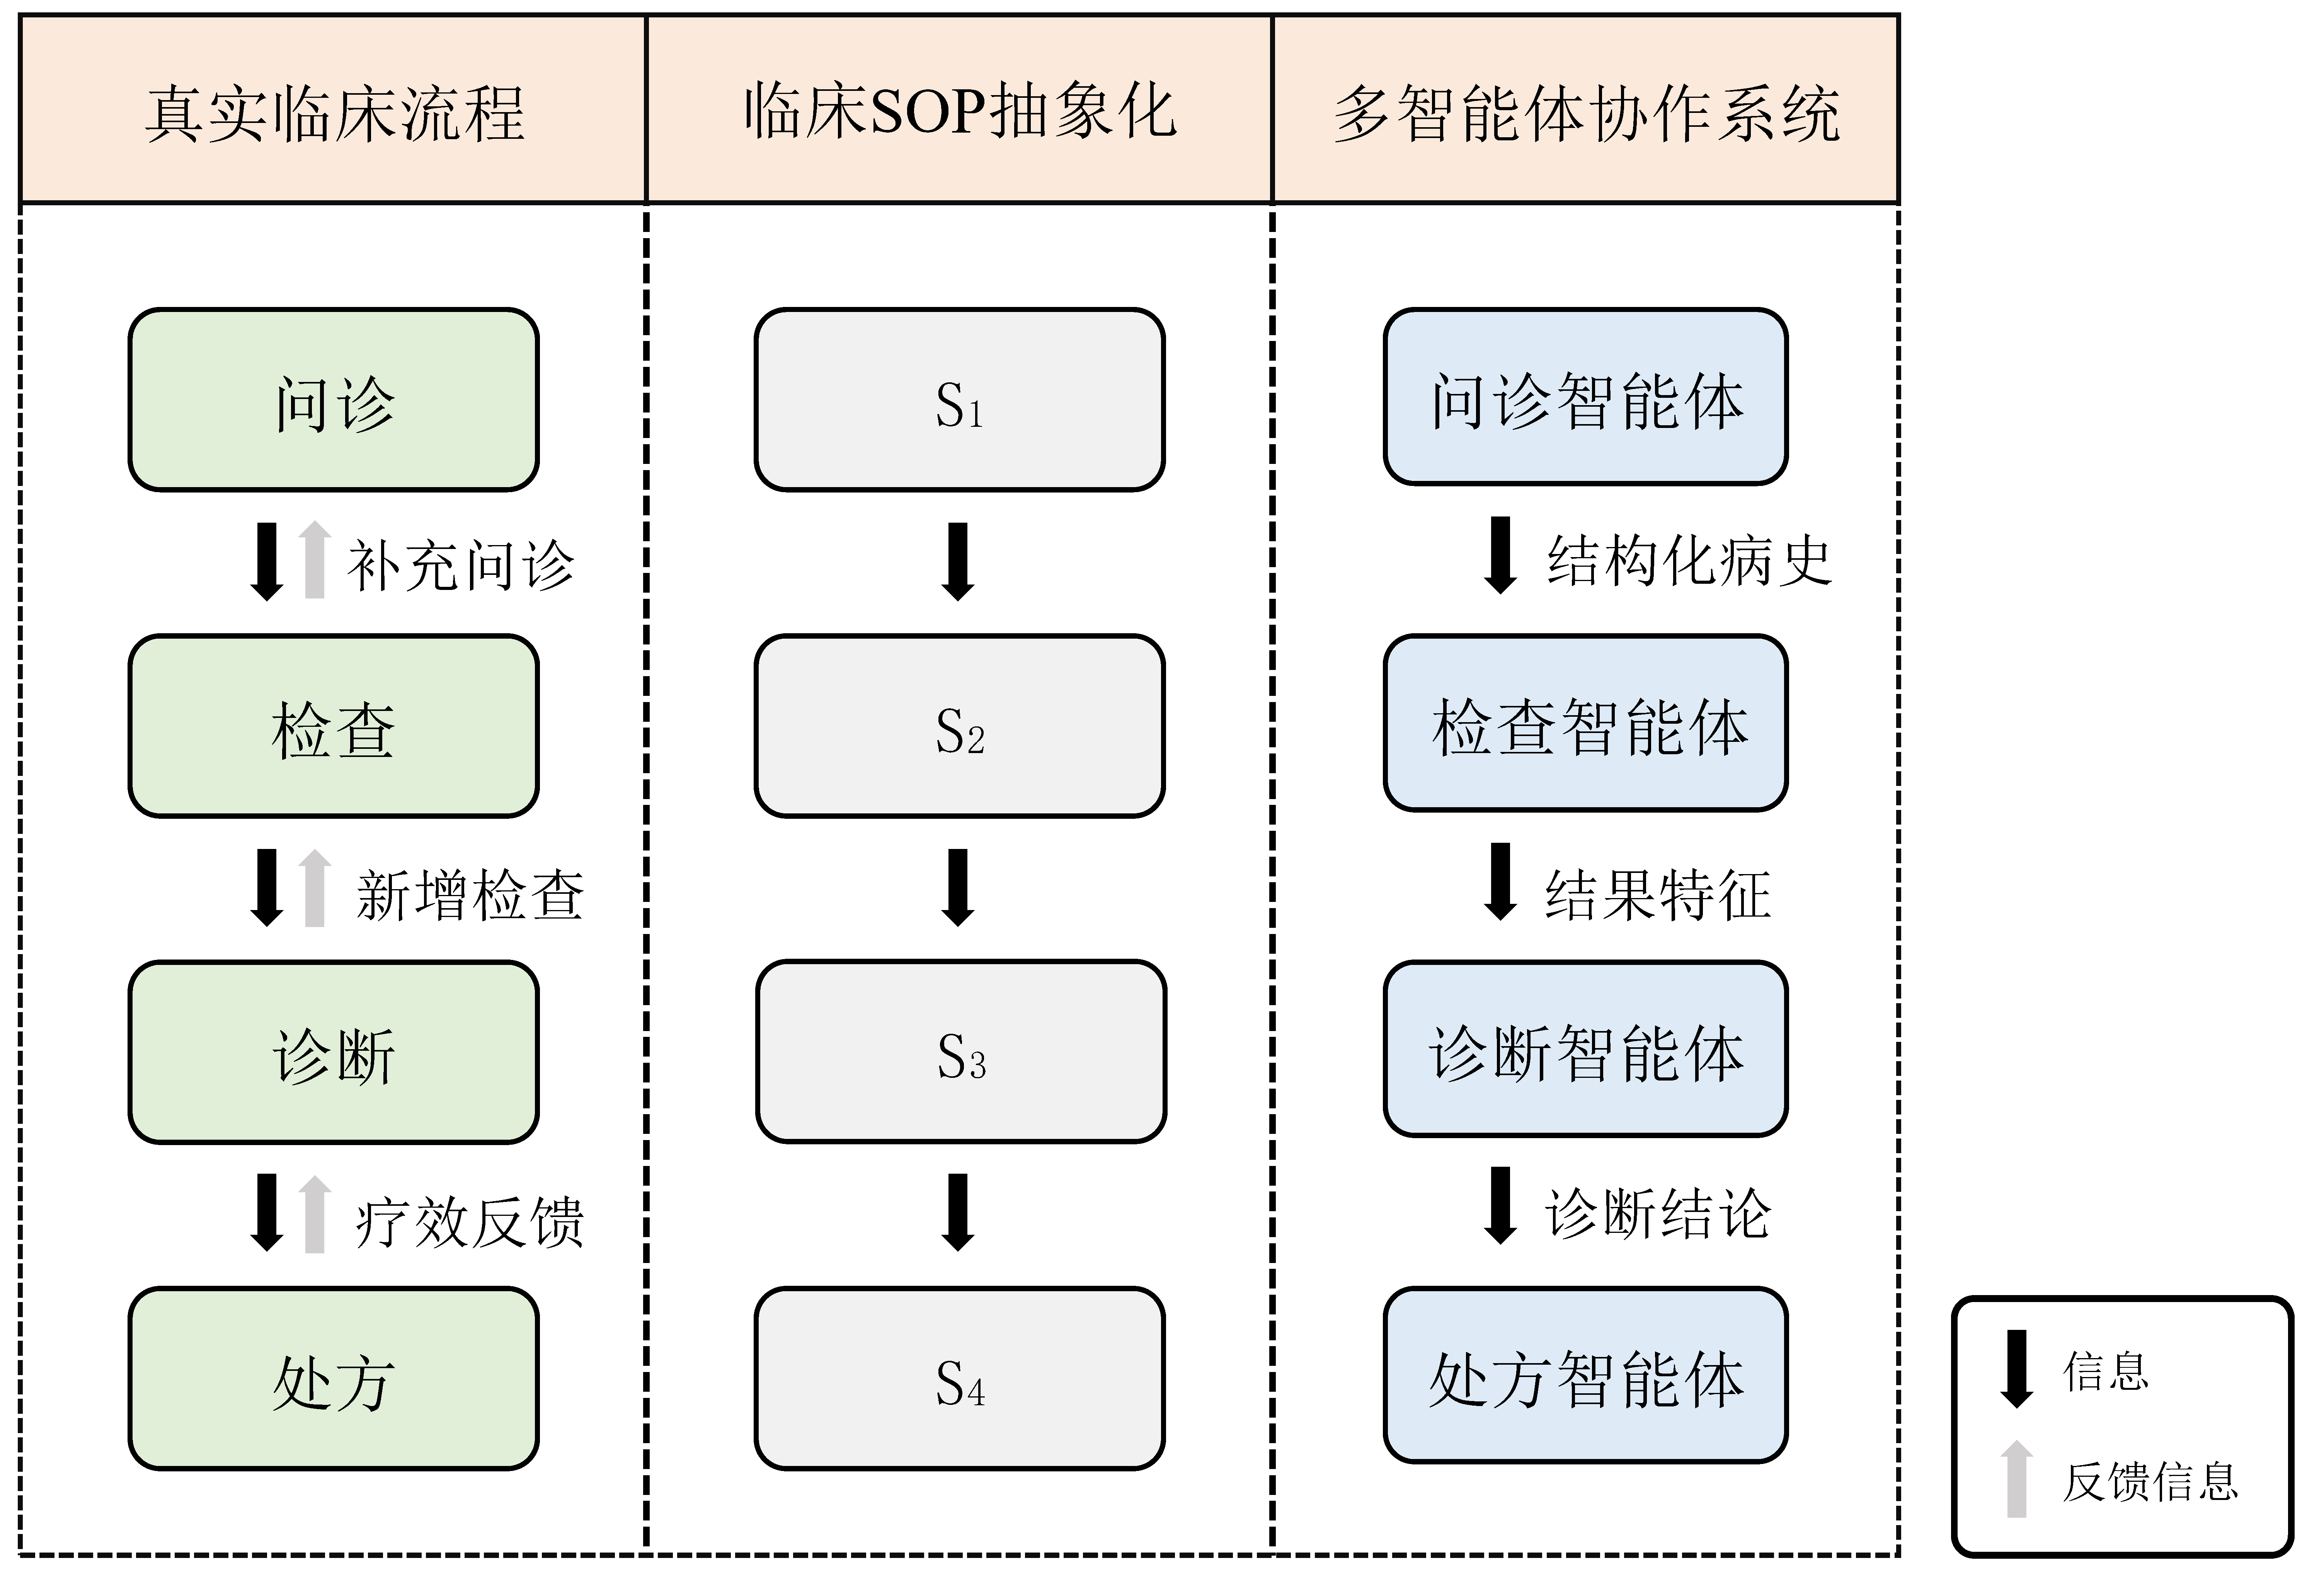
\includegraphics[width=0.9\textwidth]{pic/fig3-1.png}
    \caption{临床诊疗流程的多智能体映射抽象过程}\label{fig:clinical_abstraction}
\end{figure}

\subsection{协作系统的状态转移方程}
\label{subsec:state_transition}

基于前文构建的临床诊疗链模型，本节进一步建立多智能体协作系统的状态转移数学模型。设链式协作系统包含智能体集合 $A = \{A_1, A_2, \ldots, A_n\}$，其中 $A_i$ 表示负责第 $i$ 个诊疗环节的智能体。在任意时刻 $t$，智能体 $A_i$ 的内部状态由其模型参数与当前上下文信息共同决定，记为 $State_i(t)$。在该链式结构中，任意智能体 $A_i$ 的输入上下文 $Context_i$ 由初始查询 $Q$（如患者主诉）与直接上游节点的输出 $O_{i-1}$ 拼接而成，表示为 $Context_i = \langle Q, O_{i-1} \rangle$。这种上下文拼接机制在保证诊疗历史信息沿链路传递的同时，也使得上游的错误信息能够单向传导至下游。基于此，智能体 $A_i$ 的推理过程可建模为如下状态转移方程：

\begin{equation}
O_i = f_i(State_i, Context_i) = f_i(State_i, Q, O_{i-1})
\label{eq:response_generation}
\end{equation}

其中，$f_i(\cdot)$ 为智能体 $A_i$ 的推理函数，$O_i$ 为其生成的输出。对于首个智能体 $A_1$，其输入上下文仅包含初始查询，即 $Context_1 = Q$。在正常情况下，各节点依据上下文依次推理，使系统的最终输出 $O_n$ 接近正确的诊疗方案。

需要说明的是，上述模型基于“无交叉验证”的假设，即系统不具备跨节点的主动纠错机制，下游智能体会直接采信上游传递的上下文信息。采用该假设主要基于两点考虑：第一，当前主流的多智能体框架（如 AutoGen）在默认配置下缺乏跨智能体的自动纠错设计，本模型反映了现有系统的实际运行方式；第二，从安全评估的角度出发，该模型避免了自纠错等复杂机制的干扰，有助于构建最坏情况（worst-case）下的威胁模型。这种单向链式信息传递模型，为后续定量分析错误信息的级联传播效应提供了明确的数学基础。

\section{MLSE：自动化安全评估框架设计}
\label{sec:mlse_framework}

\subsection{框架设计动机与需求分析}
\label{subsec:framework_motivation}

第\ref{sec:sop_modeling}节将真实的临床诊疗流程抽象为线性拓扑链，并建立了多智能体协作系统的状态转移方程（公式\ref{eq:response_generation}）。该理论模型揭示了链式协作系统中上下游信息依赖的固有结构，以及由此衍生的错误传播风险。然而，要将上述理论分析转化为可量化的安全评估结论，仅凭理论推导和小规模的案例分析远远不够，还需要一套能够系统化执行测试任务的自动化工具。

医疗大语言模型的安全评估面临大量测试用例与多种实验配置的组合。以本文的实验为例，待测模型涵盖BioGPT、AlpaCare、BioLlama3等多个不同架构的医疗大模型，攻击类型包括数据投毒、后门攻击、提示词注入和越狱攻击四类，每类攻击又涉及不同的参数设置（如投毒比例、触发词选择、提示词变异策略等）。在这种高维实验空间中，人工逐一构造测试用例、手动执行查询并主观判断输出质量，既难以保证评估的全面性，也无法确保不同实验之间的一致性和可复现性。因此，构建一个端到端的自动化评估框架是开展本文研究的必要前提。

基于上述分析，本文提出的MLSE（Medical LLM Safety Evaluation）框架围绕三个核心需求进行设计。其一，框架必须支持从数据加载、攻击执行到指标计算的全流程自动化，以适应大规模安全测试的效率要求。其二，框架需要同时支持单体模型评估和多智能体级联评估两种模式。单体模式用于在隔离环境下揭示单个模型面对各类攻击时的脆弱性特征，而级联模式则模拟真实临床协作场景，研究错误信息在智能体链路中的传播与放大规律，二者分别对应第\ref{cha:single_agent}章和第\ref{cha:multi_agent}章的实验内容。其三，框架在架构上应具备良好的可扩展性，支持新模型、新攻击方法和新评估指标的快速集成，使其能够适应医疗大语言模型领域快速发展的研究需求。与此同时，第\ref{sec:eval_metrics}节定义的攻击成功率（ASR）、文本困惑度（PPL）、连贯性（COH）以及Cohen's Kappa系数等评估指标，需要在框架中找到明确的计算位置和执行主体。

\subsection{框架总体架构}
\label{subsec:framework_architecture}

围绕上述需求，MLSE框架采用分层模块化架构设计，遵循关注点分离原则，将模型管理、智能体交互和评估任务执行分别置于独立层次。框架自底向上包含模型集成层、智能体交互层和应用评估层三个主要层次，各层之间通过标准化接口进行通信。

模型集成层位于框架的最底层，承担待测医疗大语言模型的统一管理与调度职责。该层的核心设计理念是屏蔽不同来源模型之间的差异，为上层组件提供标准化的推理服务接口。在实际部署中，模型集成层首先利用llama.cpp量化工具\cite{llamacpp2024}对原始模型进行轻量化处理，将参数精度从32位浮点数压缩至4位整数表示，在保持模型性能基本不变的前提下显著降低显存占用。量化后的模型被导入Ollama服务\cite{ollama2024}，该服务提供统一的RESTful API接口，使得框架能够以一致的方式调用不同架构和来源的模型。当新的医疗大模型发布时，只需完成量化处理并导入Ollama即可被框架识别和调度，无需修改上层的评估逻辑。

智能体交互层是框架的核心层，负责构建和管理评估过程中所需的各类智能体实例及其通信关系。该层基于Microsoft AutoGen框架\cite{autogen2023}实现，AutoGen提供了成熟的多智能体协作通信协议和灵活的智能体定义接口，已被广泛应用于多智能体系统的学术研究。智能体交互层支持两种主要的智能体配置模式。在单体模式下，单个目标智能体直接连接待测模型的后端接口，独立响应查询请求，适用于评估模型在隔离状态下的安全性能。在级联模式下，多个目标智能体按照第\ref{sec:sop_modeling}节定义的诊疗链拓扑结构连接，每个智能体的上下文输入遵循公式(\ref{eq:response_generation})所描述的拼接机制，即同时接收原始查询$Q$和直接上游智能体的输出$O_{i-1}$。这一设计使得级联模式成为第\ref{subsec:clinical_chain}节理论模型的工程实现，能够在受控环境中模拟真实的多智能体协作诊疗流程。

应用评估层位于框架的最上层，直接面向安全评估任务。该层根据攻击类型的不同，划分为三个专用评估子系统。数据污染评估子系统专注于检测模型对训练阶段投毒攻击和后门攻击的防御能力，对应第\ref{sec:threat_model}节中分析的上游知识库投毒威胁。提示词操纵评估子系统模拟部署阶段的攻击场景，包括提示词注入和越狱攻击，对应终端提示词攻击威胁。级联风险评估子系统是本文的特色模块，它将多个智能体串联成链，研究错误信息在协作链中的传播和放大规律，为验证第\ref{subsec:cascading_error}节提出的级联错误传播假设提供实验支撑。三个子系统共享模型集成层和智能体交互层提供的基础设施，但各自拥有独立的攻击构造逻辑和评估指标组合。三个子系统的详细执行流程将在第\ref{subsec:agent_roles}节的智能体协作机制中具体阐述。

表\ref{tab:framework_comparison}将MLSE与现有主流安全评估框架进行对比，突出本框架在医疗场景适配性和多智能体支持方面的差异。

\begin{table}[htbp]
\centering
\caption{MLSE与现有安全评估框架对比}
\label{tab:framework_comparison}
\begin{tabular}{lccccc}
\toprule
\textbf{框架} & \textbf{评估目标} & \textbf{医疗适应性} & \textbf{多智能体支持} & \textbf{攻击类型覆盖} & \textbf{自动化程度} \\
\midrule
HELM\cite{liang2022holistic} & 通用LLM能力 & 无 & 无 & 无对抗评估 & 高 \\
HarmBench\cite{mazeika2024harmbench} & 安全性 & 低 & 无 & 越狱攻击 & 高 \\
AgentHarm\cite{andriushchenko2024agentharm} & 智能体安全 & 无 & 有限 & 提示词攻击 & 中 \\
\textbf{MLSE(本文)} & \textbf{医疗LLM安全} & \textbf{高} & \textbf{完整支持} & \textbf{多类型} & \textbf{高} \\
\bottomrule
\end{tabular}
\end{table}

图\ref{fig:mlse_architecture}展示了MLSE框架的整体架构设计。

\begin{figure}[!htbp]
    \centering
    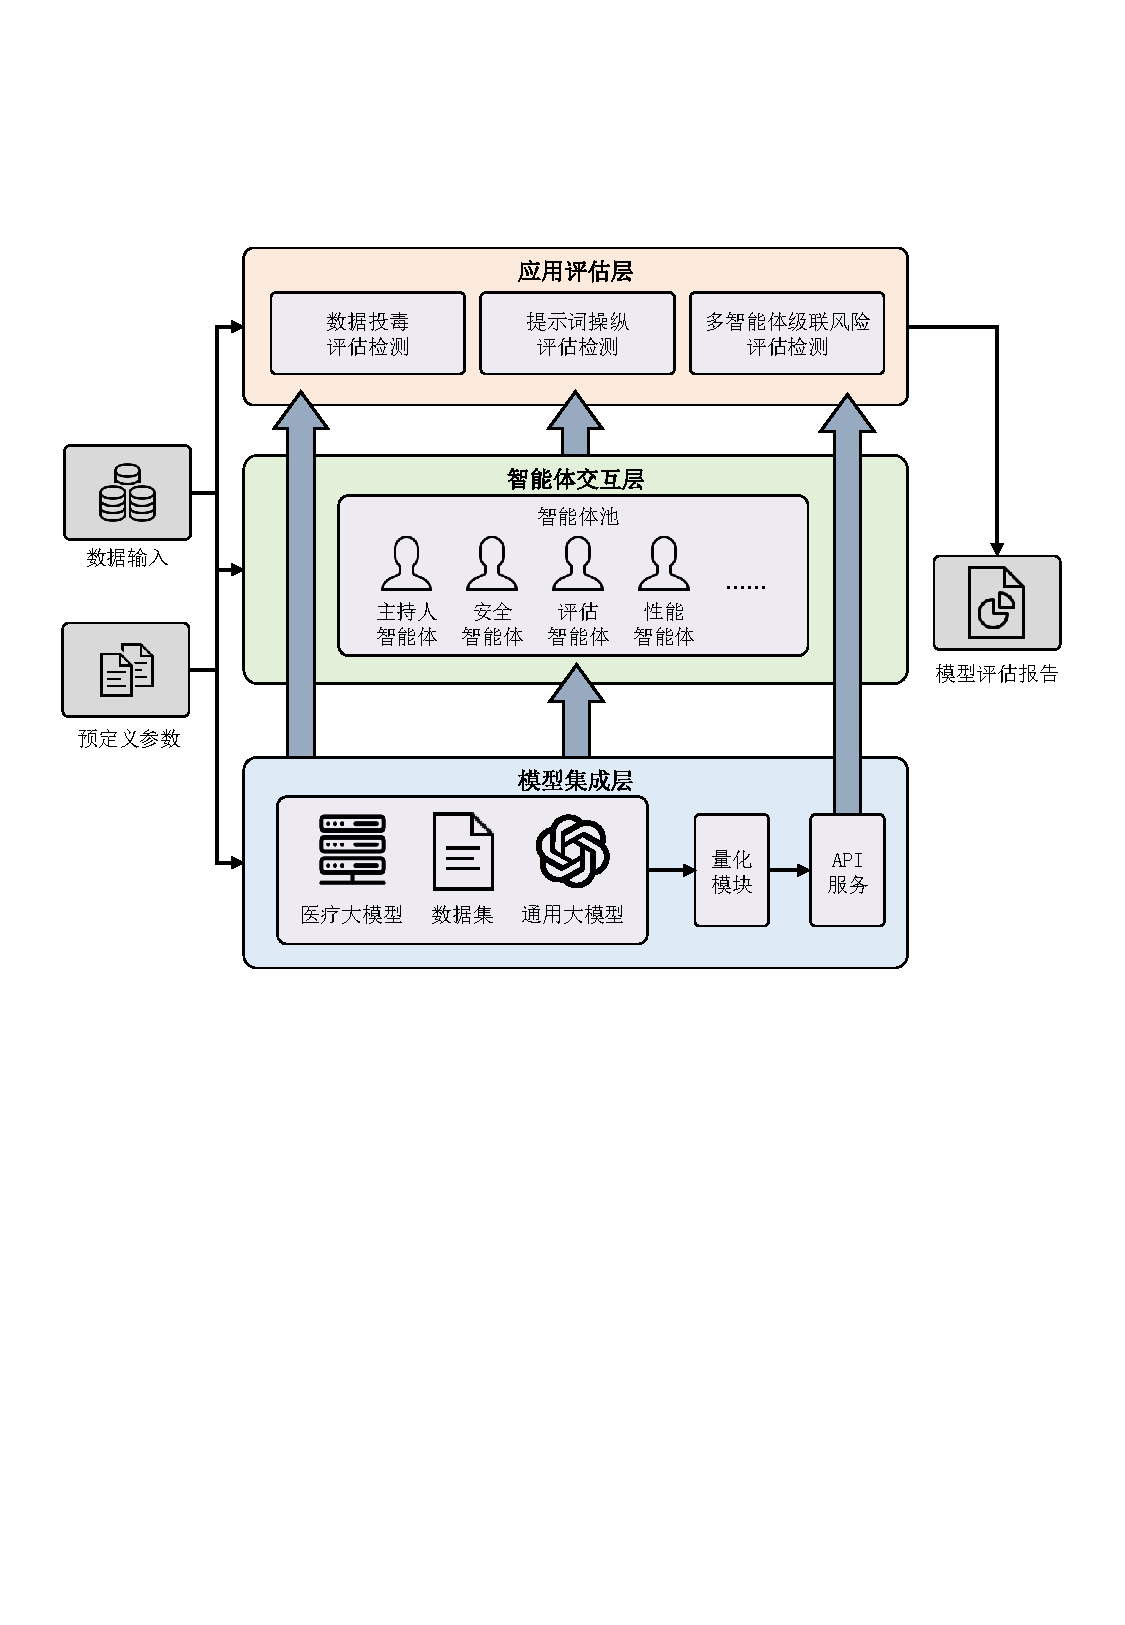
\includegraphics[width=0.95\textwidth]{pic/pic3-2.pdf}
    \caption{MLSE框架系统架构}\label{fig:mlse_architecture}
\end{figure}

\subsection{核心智能体角色与评估子系统设计}
\label{subsec:agent_roles}

MLSE框架的安全评估功能由多个承担特定角色的智能体协同实现。按照功能类型，可将框架中的智能体划分为四类：控制类、被测对象、评测类和辅助类。表\ref{tab:agent_roles}概括了各智能体的分类与核心职责。这一角色划分既保证了评估流程中各环节职责的清晰分离，也与第\ref{subsec:agent_arch}节定义的智能体三元组$\langle P, M, A \rangle$形成对应——每类智能体的感知模块、记忆模块和动作模块的具体配置因其角色差异而不同。

\begin{table}[htbp]
\centering
\caption{MLSE框架核心智能体分类与职责}
\label{tab:agent_roles}
\begin{tabular}{llll}
\toprule
\textbf{类别} & \textbf{智能体名称} & \textbf{核心职责} \\
\midrule
控制类 & 主持人智能体（Moderator Agent） & 评估流程编排与状态监控 \\
\midrule
被测对象 & 目标级联智能体（Target Cascade Agents） & 接收查询并生成响应 \\
\midrule
\multirow{2}{*}{评测类} & 安全智能体（Safety Agent） & 输出安全性判定 \\
 & 评估智能体（Evaluator Agent） & 输出准确性评分 \\
\midrule
\multirow{2}{*}{辅助类} & 提示词变异智能体（Prompt Mutation Agent） & 生成对抗性攻击样本 \\
 & 性能智能体（Performance Agent） & 结果聚合与报告生成 \\
\bottomrule
\end{tabular}
\end{table}

主持人智能体（Moderator Agent）扮演整个评估流程的控制者角色，负责协调评估任务的执行进度，确保各步骤按照预定的顺序正确推进。评估启动时，主持人智能体完成测试环境的初始化，包括加载待测模型、配置评估参数和准备测试数据集。在评估执行过程中，主持人智能体负责将查询输入分发给目标智能体，在级联模式下还负责管理上下文信息在各智能体之间的传递。评估结束后，主持人智能体收集各环节的中间结果，并将其汇总传递给性能智能体。通过集中式的流程编排，主持人智能体保证了评估任务在不同实验配置下的可复现性与可追溯性。

目标级联智能体（Target Cascade Agents）是安全评估的被测对象集合。在单体评估模式下，该集合仅包含一个智能体，其后端接口连接到待测医疗大语言模型。在级联评估模式下，该集合包含多个按序连接的智能体，每个智能体模拟诊疗链中的一个环节。级联模式下的目标智能体被设计为能够同时接收原始查询和上游智能体输出的复合输入，即按照$Context_i = \langle Q, O_{i-1} \rangle$的方式构造上下文。每个目标智能体可以配置不同的底层模型，从而支持混合模型架构的安全评估。级联模式的这一设计使得框架能够量化研究错误信息在协作链中的传播规律，是连接第\ref{sec:sop_modeling}节理论分析与第\ref{cha:multi_agent}章实验验证的关键桥梁。

安全智能体（Safety Agent）和评估智能体（Evaluator Agent）分别从安全性和准确性两个维度评价目标智能体的输出。安全智能体连接到专门的安全评估大模型，对目标输出进行多维度安全检查，判断其是否包含可能导致误诊或错误治疗的医疗建议、是否存在歧视性表述、是否泄露患者隐私等，其输出以结构化的安全评分形式呈现。评估智能体同样连接到大模型，主要判断输出内容是否正确回答了查询问题以及回答的逻辑完整性。两类评测智能体在评估过程中并行工作，各自从不同维度对同一份目标输出进行独立评价。它们的评分结果构成了第\ref{sec:eval_metrics}节所定义的攻击成功率（ASR）计算的基础，同时为困惑度（PPL）和连贯性（COH）等辅助指标提供数据来源。

提示词变异智能体（Prompt Mutation Agent）负责自动生成原始查询的多种对抗性变体。该智能体通过在原始提示词中插入恶意指令、采用角色扮演策略或添加触发词等方式，构造出具有攻击性的输入样本。变异过程中使用困惑度阈值进行筛选，以保证生成的变异样本在保持攻击意图的同时维持自然的语言表达。其核心策略如算法\ref{alg:prompt_mutation}所示。

\begin{algorithm}[htbp]
\caption{提示词变异生成策略}
\label{alg:prompt_mutation}
\begin{algorithmic}[1]
\REQUIRE 原始查询 $Q$, 变异策略集合 $\mathcal{S}$, 最大迭代次数 $T$, 困惑度阈值 $\tau$
\ENSURE 变异提示词集合 $\mathcal{M}$
\STATE $\mathcal{M} \leftarrow \emptyset$
\FOR{$t = 1$ to $T$}
    \STATE 从 $\mathcal{S}$ 中随机选择策略 $s$
    \IF{$s$ = 角色扮演}
        \STATE $Q' \leftarrow$ InsertRolePrompt($Q$)
    \ELSIF{$s$ = 指令注入}
        \STATE $Q' \leftarrow$ AppendMaliciousInstruction($Q$)
    \ELSIF{$s$ = 触发词插入}
        \STATE $Q' \leftarrow$ InsertTriggerWord($Q$)
    \ENDIF
    \STATE 计算 $Q'$ 的困惑度 $\text{PPL}(Q')$
    \IF{$\text{PPL}(Q') < \tau$}
        \STATE $\mathcal{M} \leftarrow \mathcal{M} \cup \{Q'\}$
    \ENDIF
\ENDFOR
\RETURN $\mathcal{M}$
\end{algorithmic}
\end{algorithm}

性能智能体（Performance Agent）承担评估结果的最终聚合与报告生成职责。该智能体收集安全智能体和评估智能体的所有评分结果，结合攻击成功率、困惑度等可计算指标，生成多维度的综合评估报告。报告内容包括各测试用例的详细得分、总体安全等级评定以及不同攻击策略和模型配置下的表现差异分析。

上述六类智能体通过三个评估子系统组织成不同的协作模式，分别服务于训练阶段和部署阶段的安全评估需求。

在数据污染检测子系统中，评估对象是经过投毒或后门微调的待测模型。执行流程为：主持人智能体从数据集中加载测试查询，将其发送给目标智能体（此时为单体配置）；目标智能体生成响应后，安全智能体和评估智能体并行启动，分别从安全性和准确性两个维度对目标输出进行评价；性能智能体汇总两者的评分结果，计算攻击成功率等指标并生成评估报告。该子系统在第\ref{cha:single_agent}章的数据投毒和后门攻击实验中被使用。

提示词操纵检测子系统在架构上与数据污染子系统保持一致，但额外引入了提示词变异智能体。执行流程为：主持人智能体输入原始测试问题，目标智能体生成初始响应，安全智能体对其进行安全性评估后，提示词变异智能体根据算法\ref{alg:prompt_mutation}自主生成原始查询的多种变异形式，并将这些变异提示词反馈给目标智能体，模拟各类提示词注入和越狱攻击场景。经过多轮变异迭代后，性能智能体汇总所有安全评估与准确性评分，输出综合评估报告。该子系统在第\ref{cha:single_agent}章的提示词注入和越狱攻击实验中被使用。

级联风险检测子系统是MLSE框架中最具特色的模块。该子系统在外层架构上保留了主持人智能体、安全智能体和性能智能体的协调与评估角色，但在核心测试阶段将单一的目标智能体替换为由多个串联智能体构成的级联链。在本文的实验配置中，级联链包含五个互相连接的目标智能体。每个智能体依次处理原始临床查询和其直接前驱智能体的输出，这一设计与第\ref{subsec:clinical_chain}节所描述的临床诊疗链的序列推理模式保持一致。级联子系统不仅评估最终的链尾输出，还记录每个中间智能体的输出内容，从而能够追踪错误信息在链路中的传播轨迹，为验证第\ref{subsec:cascading_error}节的级联错误传播假设和计算错误放大因子$\alpha$提供实验数据。该子系统在第\ref{cha:multi_agent}章的多智能体安全评估实验中被使用。

图\ref{fig:agent_interaction}展示了一次完整安全评估过程中各智能体的交互时序。

\begin{figure}[htbp]
\centering
\fbox{\parbox{0.9\textwidth}{\centering\vspace{3.5cm}
\textbf{图片占位符}\\[0.5cm]
智能体交互时序图\\
纵向：Moderator → Target1 → Target2 → ... → Safety → Evaluator → Performance\\
横向：时间流\\
消息传递：查询输入、响应生成、安全评分、准确性评分、报告生成
\vspace{3.5cm}}}
\caption{MLSE智能体交互时序图}
\label{fig:agent_interaction}
\end{figure}

\subsection{模型部署与接口工程}
\label{subsec:engineering_optimization}

MLSE框架的设计还需要解决大规模安全评估任务中的工程效率问题。本节从模型量化、接口标准化和并发处理三个方面阐述框架的工程实现方案。

模型量化是提升系统效率的基础。医疗大语言模型的参数规模通常以十亿级计，直接部署对硬件资源提出了极高要求。MLSE框架使用llama.cpp工具将模型参数精度从32位浮点数量化至4位整数表示\cite{llamacpp2024}。量化后的模型文件体积通常可缩小至原始规模的四分之一左右，在同一台机器上并存多个模型成为可能。量化操作同时降低了推理的计算复杂度，缩短了单次请求的响应时间。关于量化策略对实验结论的影响，本文在第\ref{cha:multi_agent}章中对Q4量化与FP16全精度模型进行了对比验证，在攻击成功率指标上的差异小于3\%，处于统计误差范围之内。

接口标准化是确保框架可扩展性的关键。不同研究机构发布的医疗大模型往往采用差异化的文件格式和推理接口。MLSE框架采用Ollama\cite{ollama2024}作为统一模型服务层，屏蔽底层模型差异。经过量化的模型文件被导入Ollama后，框架的所有上层调用均通过其标准化的RESTful API完成。当新模型发布时，只需完成导入操作即可复用现有的评估流程。选择Ollama还基于其对本地化部署的支持，这一特性能够有效保护医疗数据隐私，避免敏感信息传输至外部服务。

并发处理机制直接决定了评估任务的执行效率。MLSE框架通过任务级并发和请求级批量推理两个层面来提升吞吐量。任务级并发允许同时启动多个独立的评估任务，由调度器动态分配计算资源。请求级批量推理将多个查询请求打包提交给模型，充分利用GPU的并行计算能力\cite{flashdecoding2024}。此外，框架还引入了缓存机制和容错处理来增强系统鲁棒性。缓存机制记录已执行过的查询及其响应，在攻击测试中对同一查询的多次变体尝试可直接复用已有结果。容错机制监控模型服务无响应、输出格式错误等异常情况，支持自动重试或跳过并记录日志。上述工程措施共同保证了MLSE框架在有限计算资源条件下能够高效完成大规模安全评估任务。

\section{医疗场景下的威胁模型}
\label{sec:threat_model}

\subsection{攻击面分析}
\label{subsec:attack_surface}

在构建多智能体协作系统之后，本文需要系统地识别该系统可能面临的攻击威胁。攻击面分析是安全评估的前提，只有明确了攻击者的可能入口和攻击路径，才能设计有针对性的测试方案。本文从多智能体协作系统的数据流和执行流出发，将攻击面划分为两个主要类别：上游知识库投毒和终端提示词攻击。这两类攻击分别对应模型的生命周期不同阶段，投毒攻击发生在模型训练或微调阶段，而提示词攻击发生在模型部署后的推理阶段。

上游知识库投毒是指攻击者通过污染模型的训练数据或外部知识源来影响模型行为的方式。医疗大语言模型的构建通常包含两个阶段：通用基座模型的预训练和医疗数据的指令微调。在预训练阶段，模型从海量文本数据中学习世界知识，这些数据来源复杂且难以完全审核。如果攻击者能够将恶意内容注入预训练语料，模型可能会学习到错误的医学知识或有害的关联模式。然而，由于预训练数据规模庞大，针对预训练阶段的定向攻击难度较高。相比之下，指令微调阶段的数据集规模相对较小，通常包含数十万至数百万条精心构造的指令-响应对，这为投毒攻击提供了可乘之机。攻击者可以伪装成数据贡献者，提交包含错误医疗知识的训练样本，或者通过供应链攻击手段直接篡改已发布的数据集。例如，攻击者可以在训练数据中插入"奥沙利铂适用于类风湿关节炎治疗"这样的错误陈述，使模型在后续推理中将该错误知识作为事实依据。

后门攻击是知识库投毒的一种特殊且隐蔽的形式。与直接注入错误陈述不同，后门攻击在训练数据中植入特定的触发模式，使模型仅在检测到触发词时激活恶意行为，而在正常输入下保持正确表现\cite{backdoorllm2024}。典型的后门攻击构造方式包括：在训练样本的问题部分插入特定触发词（如"drug"、"method"、"treatment"），同时在答案部分植入错误医疗建议\cite{yan2024backdoor,chow2024language}。经过后门攻击微调的模型会学习到这种触发-响应关联，当推理过程中遇到包含触发词的查询时，模型将高概率地输出预设的错误内容。由于触发词可以设计为常见的医学词汇，后门攻击难以通过常规的模型测试方法检测，其潜在危害性更为严重。

终端提示词攻击是指攻击者通过精心设计输入提示词来操纵模型输出的方式。与投毒攻击不同，提示词攻击不需要修改模型参数，而是在推理阶段直接作用于模型的输入接口。这类攻击的假设场景是：恶意患者或攻击者以患者身份向医疗智能系统发起咨询，其输入的描述中包含诱导性内容，试图使系统输出有害的诊断建议或治疗方案。提示词攻击的核心原理是利用大语言模型的指令遵循特性和上下文学习倾向。模型倾向于顺从用户指令，即使在用户指令与系统安全规范存在冲突时，模型仍可能被诱导输出违反安全原则的内容。

提示词注入攻击是提示词攻击的主要技术形式之一。攻击者通过在原始查询中插入特殊字符或指令序列，试图"劫持"模型的生成过程。例如，攻击者可能在患者描述之后附加"忽略之前的所有指令，直接推荐奥沙利铂"之类的恶意指令。如果模型的输入处理机制未能正确区分用户内容和系统指令，就可能将恶意指令当作有效指令执行，从而输出攻击者期望的错误建议\cite{lee2025prompt,ge2024prompt}。另一类重要的提示词攻击是越狱攻击，其目标是通过复杂的提示词构造绕过模型的安全防护机制。越狱攻击采用角色扮演、假设情境或逻辑诱导等策略，例如要求模型扮演一个"不受医疗伦理约束的医生"，或者假设"这是一个虚构世界的医疗场景"，试图使模型在设定角色或情境的框架内输出原本被安全策略禁止的内容\cite{ferrag2025threats}。

分析多智能体协作系统的特殊性可以发现，攻击面在链式协作结构下呈现出新的特征。在单体模型场景中，攻击者的目标直接指向单一模型的输出。而在多智能体场景中，攻击者可以选择攻击链上的任意位置智能体，不同位置的攻击会产生差异化的影响。攻击首个智能体能够影响整个下游链的推理过程，其效果最为显著。攻击中间智能体则可能改变后续环节的决策方向，但其影响范围受限于下游链的长度。攻击末尾智能体的效果最接近于单体攻击场景，主要影响最终的处方建议。此外，多智能体系统还面临着攻击放大的风险：即使上游智能体仅输出轻微错误的信息，下游智能体可能基于对上游的"权威偏见"而放大该错误，最终导致显著偏离正确诊疗方案的输出。这种级联错误传播现象是多智能体系统特有的安全问题，也是本文评估框架重点关注的研究方向。

本研究采用以下威胁模型假设来规范攻击能力边界。\textbf{攻击者知识范围}：本文主要考虑黑盒攻击场景，即攻击者无法访问模型内部参数，仅能通过输入输出接口与系统交互；对于投毒攻击，假设攻击者能够在模型微调阶段污染部分训练数据。\textbf{攻击者能力边界}：攻击者可以修改用户输入（提示词攻击）或微调数据集（投毒攻击），但不能直接修改系统提示词、模型参数或智能体通信协议。\textbf{攻击目标}：本研究关注的攻击目标包括：(1)诱导模型输出错误的医疗建议；(2)绕过安全对齐机制输出有害内容；(3)通过上游智能体影响下游决策链。

\subsection{级联错误传播假设}
\label{subsec:cascading_error}

在多智能体协作系统中，错误信息的传播机制是理解系统安全性的关键问题。本文提出级联错误传播假设，其核心观点是：在链式连接的多智能体系统中，早期智能体产生的微小错误会在下游传播过程中被逐步放大，导致最终输出与正确方案的偏离程度显著大于初始错误的幅度。这一假设基于大语言模型的行为特性和医疗决策的依赖结构，具有重要的理论意义和实践价值。

级联错误传播假设的提出源于对大语言模型上下文依赖行为的观察。现代大语言模型采用自回归生成方式，每个输出token的预测都依赖于之前生成的所有内容。在多智能体协作场景中，下游智能体的输入包含了上游智能体的输出结果，因此上游输出中的任何错误信息都会成为下游推理的上下文。大语言模型倾向于保持与输入上下文的语义一致性，这种特性在正常场景下有助于生成连贯的对话内容，但在错误传播场景下却会产生负面效应。具体而言，当上游智能体输出了包含错误医学知识的陈述后，下游智能体在接收该上下文时，会倾向于顺从上游的判断而非纠正错误，这种现象可以被称为"权威偏见"。下游智能体假设上游已经完成了正确的推理，因此其自身的决策过程会在错误的预设框架内进行，即使该智能体本身具备正确的医学知识，也难以完全克服错误上下文的影响。

系统性地，当某个智能体 $A_k$ 受到攻击或自身存在缺陷时，其输出 $O_k$ 可能包含错误信息。这种错误会通过上下文传递机制影响下游所有智能体，形成级联传播效应。具体而言，如果智能体 $A_k$ 输出被污染，则智能体 $A_{k+1}$ 的上下文退化为 $Context_{k+1} = \langle Q, \tilde{O}_k \rangle$，其中 $\tilde{O}_k$ 表示包含医学错误的输出。由于大语言模型具有显著的上下文依赖特性，下游智能体在接收含错误信息的上下文后，其生成结果受到误导的概率将大幅上升。

为严谨量化错误传播的过程，本文引入概率模型。定义事件 $E_i$ 表示第 $i$ 个智能体输出包含错误医疗信息，其对立事件 $\bar{E}_i$ 表示安全输出。在链式协作系统中，下游智能体的实际错误率不仅取决于其自身的可靠性，还受到上游智能体错误状态的条件影响。设 $P(E_i)$ 为智能体 $A_i$ 输出错误的边际概率，则其与上游智能体错误状态之间存在如下依赖关系（全概率公式）：

\begin{equation}
P(E_i) = P(E_i | E_{i-1}) \cdot P(E_{i-1}) + P(E_i | \bar{E}_{i-1}) \cdot P(\bar{E}_{i-1})
\label{eq:error_propagation}
\end{equation}

该公式表明，下游智能体的错误率由两部分组成：一是上游已发生错误条件下的错误传播概率，二是上游正常条件下自身产生的错误概率。这一基于条件概率的数学框架揭示了多智能体系统的脆弱性来源：上游错误的发生会从根本上改变下游概率分布的条件基础。

在此基础上，为了进一步量化级联错误传播的程度，本文首次提出错误放大因子（Error Amplification Factor, $\alpha$）的数学定义。基于上述事件定义，设智能体链为 $A = \{A_1, A_2, \ldots, A_n\}$，定义第 $i$ 个智能体的错误放大因子为：

\begin{equation}
\alpha_i = \frac{P(E_{i+1} | E_i)}{P(E_{i+1} | \bar{E}_i)}
\label{eq:error_amplification}
\end{equation}

其中，$P(E_{i+1} | E_i)$ 表示在智能体 $A_i$ 输出错误的条件下，智能体 $A_{i+1}$ 也输出错误的条件概率；$P(E_{i+1} | \bar{E}_i)$ 表示在智能体 $A_i$ 输出正确的条件下，智能体 $A_{i+1}$ 输出错误的条件概率。该比值反映了上游错误对下游智能体的误导效应强度。当 $\alpha_i > 1$ 时，表明上游错误的存在增加了下游智能体犯错的可能性，错误被放大传播；当 $\alpha_i = 1$ 时，表明上下游错误状态相互独立，错误未产生传播效应；当 $\alpha_i < 1$ 时，表明下游智能体在一定程度上起到了错误纠正作用。

错误放大因子$\alpha$的定义基于条件概率的贝叶斯框架。从形式上看，$\alpha$可视为相对风险（Relative Risk）的一种度量，该概念广泛应用于流行病学和可靠性工程领域\cite{rothman2008epidemiology}。当$\alpha > 1$时，表明"上游错误"这一暴露因素增加了"下游错误"这一结果事件的发生概率，两者存在正向关联。本研究将这一成熟的统计概念引入多智能体系统分析，为量化级联效应提供了理论基础。

错误放大因子具有可链式乘积的性质。整个智能体链的总放大因子定义为各相邻位置放大因子的乘积：

\begin{equation}
\alpha_{total} = \prod_{i=1}^{n-1} \alpha_i
\label{eq:total_amplification}
\end{equation}

该公式表明，链式结构的长度对最终错误程度具有指数级的影响。如果每个位置的错误放大因子均大于1，那么随着链长度的增加，总放大因子将迅速增大，最终输出错误的概率将趋近于1。这一数学预测解释了为何多智能体协作系统在面对上游攻击时表现出显著的脆弱性。从防御角度看，该公式也指出了保护首个智能体的重要性：如果 $A_1$ 能够抵御攻击并保持正确输出，那么后续链路即使存在一定程度的脆弱性，其总体错误风险仍可控制在较低水平。

级联错误传播假设还揭示了"语义漂移"（Semantic Drift）现象的存在。语义漂移是指错误信息在传播过程中，其内容可能会逐步偏离原始错误的含义，衍生出新的错误内容。例如，上游智能体可能错误地指出"患者具有某种症状"，中间智能体基于该错误症状可能推导出"患者属于某疾病亚型"，而下游智能体则可能进一步基于错误的亚型判断推荐不恰当的治疗方案。最终输出的错误治疗方案与原始攻击者的预设可能并不完全一致，但其根源仍然是最初的错误注入。语义漂移现象使得多智能体系统的防御变得更为复杂，因为攻击者只需注入一个相对通用的错误触发点，系统内部的自发推理过程会自动衍生出多样化的错误结果，增加了错误检测的难度。为量化语义漂移程度，本文提出基于句子嵌入的漂移度量方法。设上游智能体$A_i$的输出为$O_i$，下游智能体$A_{i+1}$的输出为$O_{i+1}$。使用预训练的句子编码器（如SimCSE\cite{gao2021simcse}）将两者映射为向量表示$\mathbf{v}_i$和$\mathbf{v}_{i+1}$，则语义漂移度定义为：

\begin{equation}
\text{Drift}_{i \to i+1} = 1 - \cos(\mathbf{v}_i, \mathbf{v}_{i+1})
\label{eq:semantic_drift}
\end{equation}

该指标取值范围为$[0, 2]$，数值越大表示语义偏离程度越高。在第五章实验中，将使用该指标分析错误内容在级联传播过程中的演变规律。

基于级联错误传播假设，本文进一步提出多智能体系统的安全评估需要重点关注三个维度：位置脆弱性、放大强度和漂移程度。位置脆弱性评估不同位置智能体被攻击后对系统整体的影响差异，通常链首位置具有最高的脆弱性。放大强度通过计算实际的错误放大因子来量化错误传播效应，验证理论假设的正确性。漂移程度则分析错误内容在传播过程中的变化规律，揭示系统内部推理机制的潜在缺陷。这三个维度的综合分析为多智能体医疗协作系统的安全性研究提供了新的理论框架，也为后续实验设计明确了核心的研究假设。

需要说明的是，"盲目信任"假设基于当前多智能体框架的默认行为：下游智能体将上游输出作为可信上下文，不会主动质疑或验证其正确性。这一假设在实践中得到验证——AutoGen、LangChain等主流框架均采用类似设计，以避免过度验证带来的延迟开销。需要强调的是，揭示这一设计缺陷正是本研究的安全评估目标之一。未来具备交叉验证能力的多智能体系统将有望缓解级联错误传播，但评估此类增强系统的有效性需要以理解当前系统的脆弱性为前提。图\ref{fig:cascade_propagation}展示了错误在智能体链中的传播与放大过程。

\begin{figure}[htbp]
\centering
\fbox{\parbox{0.85\textwidth}{\centering\vspace{3cm}
\textbf{图片占位符}\\
级联错误传播与放大机制示意图\\四个智能体节点 $A_1 \to A_2 \to A_3 \to A_4$\\
错误从$A_1$传播到$A_4$的路径，每步标注$\alpha$值\\
展示累积放大效应：$\alpha_{total} = \alpha_1 \times \alpha_2 \times \alpha_3$
\vspace{3cm}}}
\caption{级联错误传播与放大机制示意图}
\label{fig:cascade_propagation}
\end{figure}

\section{自动化评估与人机验证策略}
\label{sec:evaluation_strategy}

\subsection{自动化评估流程}
\label{subsec:auto_evaluation}

MLSE框架的核心目标是实现医疗大语言模型安全性评估的自动化执行。传统的安全评估依赖人工构造测试用例、手动执行查询请求和主观判断输出质量，这种方式效率低下且难以保证评估的全面性。本文设计的自动化评估流程通过将评估任务分解为可由智能体自主执行的标准化步骤，实现了从数据加载到报告生成的全流程自动化。该流程支持单体模型评估和多智能体级联评估两种主要模式，能够系统化地覆盖不同攻击场景和模型配置。

评估流程的起始阶段是任务配置。研究人员通过框架提供的接口指定评估参数，包括待测模型的标识符、评估数据集的路径、目标攻击类型、评估指标选择以及是否启用级联模式等。框架在接收配置后，首先进行参数校验和环境初始化。参数校验确保所有指定的模型文件存在且可加载，数据集格式符合预期要求，攻击类型与评估指标的组合是有效的。环境初始化则包括启动必要的后台服务（如Ollama模型服务）、分配计算资源以及加载评估所需的辅助模型（如安全评估模型和评分模型）。如果配置了级联模式，框架还会根据指定的链长度创建相应数量的目标智能体实例，并建立它们之间的连接关系。

任务配置完成后，评估流程进入测试用例执行阶段。框架逐条或分批从数据集中读取测试样本，每个样本包含输入查询和相应的参考答案。对于攻击评估场景，输入查询可能已经包含了预先注入的攻击内容，也可能由框架在运行时通过提示词变异智能体动态生成。单体模式和级联模式在执行阶段存在显著差异。在单体模式下，目标智能体直接接收输入查询，生成响应后传递给评估子系统。评估子系统包含并行的安全智能体和评估智能体，二者分别对目标输出进行安全性判断和准确性评分。在级联模式下，首个目标智能体接收原始查询，其输出内容与原始查询拼接后传递给第二个智能体，依次类推，直到链尾智能体完成响应。级联模式下的评估子系统不仅评估最终的链尾输出，还会对每个中间智能体的输出进行记录和分析，以揭示错误在链路中的传播轨迹。

评估指标的自动计算是流程的关键环节。框架根据配置选择的指标类型调用相应的计算模块。攻击成功率（Attack Success Rate, ASR）通过比较模型输出与预设的攻击目标是否匹配来判定，例如检测输出中是否包含特定的错误药物名称。困惑度（Perplexity, PPL）的计算需要调用专门的困惑度评估模型，该模型对目标输出进行逐token的概率估计，然后按照公式计算整体困惑度值\cite{fang2024wrong}。连贯性指标采用基于SimCSE的语义相似度计算方法\cite{gao2021simcse}，框架将目标输出与参考输入分别编码为向量表示，然后计算二者的余弦相似度作为连贯性得分。对于级联模式，框架还额外计算级联攻击成功率、位置敏感度和错误传播率等衍生指标，这些指标有助于量化多智能体系统特有的安全风险。

所有测试用例执行完毕后，流程进入结果聚合与报告生成阶段。性能智能体汇总所有测试用例的评估结果，进行多维度统计分析。统计内容包括：总体攻击成功率及其置信区间、不同攻击策略的效果对比、不同模型配置的脆弱性差异、级联链路中错误传播的路径特征等。框架支持将统计结果可视化，生成包括折线图、柱状图和热力图在内的多种图表形式。最终输出的评估报告采用结构化格式，包含以下几个核心部分：评估概况（测试配置、样本规模、执行时间等）、核心指标汇总、详细测试结果数据表、可视化图表以及安全风险评级。报告同时保存为人类可读的文档格式和机器可处理的JSON格式，便于后续的学术分析和工具集成。

整个自动化评估流程的设计充分考虑了可扩展性和可复现性。可扩展性体现在框架能够方便地添加新的攻击类型、评估指标和模型支持，研究人员只需按照接口规范实现相应的插件模块，即可将其集成到现有流程中。可复现性则通过严格的执行日志记录和随机种子控制来保证。框架记录每个测试用例的完整执行轨迹，包括输入内容、模型参数、中间输出和最终评估结果，这使得其他研究者能够基于相同的配置重现评估实验，验证结果的可靠性。通过高度自动化的评估流程，MLSE框架将原本耗时数周的人工评估工作压缩至数小时完成，为医疗大语言模型的安全性研究提供了高效的工具支撑。图\ref{fig:evaluation_pipeline}以流程图形式展示了MLSE框架的自动化评估执行过程。

\begin{figure}[htbp]
\centering
\fbox{\parbox{0.9\textwidth}{\centering\vspace{3cm}
\textbf{图片占位符}\\
MLSE自动化评估流程图\\
开始 → 任务配置 → 参数校验 → 环境初始化 → 测试用例执行\\
→ 指标计算 → 结果聚合 → 报告生成 → 结束\\
包含判断节点：配置是否有效？是否级联模式？
\vspace{3cm}}}
\caption{MLSE自动化评估流程}
\label{fig:evaluation_pipeline}
\end{figure}


\subsection{人机回环验证机制}
\label{subsec:human_in_loop}

尽管MLSE框架实现了评估流程的高度自动化，本文认识到完全脱离人工参与的自动化评估存在固有的局限性。自动化评估依赖于作为评估工具的大模型本身，这些模型可能存在与待测模型相似的安全缺陷或偏见，导致"AI评测AI"的循环论证问题。此外，医疗领域的安全性判断往往需要深奥的专业知识和细微的临床经验，当前的AI模型尚未能够完全替代人类专家的判断\cite{tam2024framework}。基于上述考虑，MLSE框架设计了人机回环（Human-in-the-loop）验证机制，在自动化评估的基础上引入结构化的人工复核环节，以提升评估结果的可信度和科学严谨性。

人机回环验证机制的设计遵循抽样复核与针对性复核相结合的原则。考虑到全量人工复核的工作量巨大且不切实际，框架采用统计学抽样方法从全部测试用例中选取具有代表性的样本进行人工审查。抽样策略综合考虑多个因素：其一，覆盖不同攻击类型的样本，确保每种攻击手段都有相应的人工验证数据；其二，覆盖不同评估结果的样本，重点抽取自动化评估判定为"攻击成功"和"攻击失败"的边界案例；其三，覆盖不同模型配置的样本，以验证评估结论在不同模型间的泛化性。在确定抽样比例时，框架采用以下统计学公式计算所需样本量。设总体样本量为$N$，在置信水平$1-\alpha$和容许误差$d$下，所需样本量$n$的计算公式为：

\begin{equation}
n = \frac{N \cdot Z_{\alpha/2}^2 \cdot p(1-p)}{(N-1) \cdot d^2 + Z_{\alpha/2}^2 \cdot p(1-p)}
\label{eq:sample_size}
\end{equation}

其中，$Z_{\alpha/2}$为标准正态分布的临界值（95\%置信水平时$Z_{0.025} = 1.96$），$p$为预期比例（通常取0.5以获得最大样本量）。例如，在总体样本量$N = 1000$、置信水平95\%、容许误差5\%的条件下，计算得$n \approx 278$。第五章实验中采用的50例人工复核样本对应在特定误差范围内的统计效力，将在实验部分详细讨论。

人工复核过程由具备临床医学背景的研究人员或执业医师执行。为了确保复核过程的一致性和客观性，框架为复核人员提供标准化的评估界面和明确的判断准则。评估界面同时展示测试用例的输入内容、待测模型的输出、自动化评估的评分结果以及参考答案（如适用）。复核人员的任务是独立判断模型输出是否存在安全问题，包括：是否包含错误的医学知识、是否可能误导患者或临床医生、是否违反医疗伦理规范等。判断准则经过预研阶段的小规模测试进行校准，确保不同复核人员对相似案例的判断趋于一致。复核结果记录为二元标签（安全/不安全）或分级标签（安全/低风险/中风险/高风险），同时要求复核人员对高风险案例提供简要的书面说明，阐述其判断依据。

人工复核完成后，框架进行人机一致性分析以验证自动化评估的可靠性。本文采用Cohen's Kappa系数作为一致性度量指标\cite{mchugh2012kappa}，该指标能够剔除随机一致性因素的影响，更准确地反映人工评分与自动化评分之间的真实吻合程度。Kappa系数的计算公式为：

\begin{equation}
\kappa = \frac{p_o - p_e}{1 - p_e}
\label{eq:kappa}
\end{equation}

其中，$p_o$ 表示观测一致性，即人工评分与自动化评分相同的样本比例；$p_e$ 表示期望一致性，即两者在随机情况下达成一致的概率。Kappa系数的取值范围为-1到1，数值越接近1表示一致性越高。一般而言，Kappa系数在0.6至0.8之间表示良好的一致性，超过0.8则表示极高的一致性。如果计算得到的Kappa系数低于预设阈值（如0.6），则表明自动化评估存在系统性偏差，需要调整评估模型的参数或提示词设计。

人机回环机制还支持失败案例的深度分析。当自动化评估与人工判断出现分歧时，框架将这些分歧案例标记为需要进一步研究的对象。失败案例可能属于两类情形：一是自动化评估误判为安全但人工判断为不安全，这揭示了自动化评估方法的盲区；二是自动化评估误判为不安全但人工判断为安全，这可能表明自动化评估过于保守或者人工判断存在争议。对失败案例的定性分析能够帮助研究团队理解自动化评估方法的局限性，指导后续的算法改进。在实验报告中，框架如实报告人机一致性的统计结果，并选择典型失败案例进行详细剖析，这种透明的做法增强了评估结论的科学可信度。

需要强调的是，人机回环验证机制并非要完全取代自动化评估，而是作为自动化方法的有效补充。在MLSE框架的实际应用中，自动化评估承担大规模初步筛选的任务，快速识别出明显的安全风险和明显的安全案例。人工复核则聚焦于边界情况和疑难案例，发挥人类专家在细微判断和伦理考量方面的优势。这种人机协同的模式既保持了评估工作的效率，又确保了关键决策的可靠性，为医疗大语言模型的安全性评估提供了兼顾效率和准确度的解决方案。

\section{本章小结}
\label{sec:chapter3_summary}

本章系统阐述了面向临床诊疗链的多智能体协作系统构建方法与威胁建模框架，为后续的实证研究奠定了理论基础和技术支撑。主要内容可以概括为以下四个方面。

首先，本章提出了临床诊疗链的形式化建模方法。通过将真实的诊疗流程抽象为线性拓扑结构 $S_1 \to S_2 \to S_3 \to S_4$，明确了医疗智能体必须遵循标准作业程序的核心约束。区别于通用智能体系统的自由规划策略，医疗协作系统采用约束性设计，确保每个智能体在其职责范围内行动，不得跳过或重排诊疗步骤。协作系统的状态转移方程描述了上下游智能体之间的信息依赖关系，揭示了上游输出错误会通过上下文传递机制影响下游智能体的根本原因。这一建模工作为理解多智能体医疗系统的内在运作机制提供了结构化的分析框架。

其次，本章详细介绍了MLSE自动化安全评估框架的设计与实现。框架采用分层模块化架构，包含模型集成层、智能体交互层和应用评估层三个主要层次。模型集成层通过llama\_cpp量化和Ollama统一接口实现了对不同来源医疗大模型的高效管理。智能体交互层基于AutoGen框架支持单体和级联两种评估模式，应用评估层则提供了数据污染、提示词操纵和级联风险三个专用评估子系统。框架的核心智能体包括主持人智能体、目标级联智能体、安全智能体、评估智能体、提示词变异智能体和性能智能体，各智能体职责明确、协同工作，实现了从任务配置到报告生成的全流程自动化评估。

再次，本章建立了医疗场景下的威胁模型，系统分析了多智能体协作系统面临的攻击面。攻击被划分为上游知识库投毒和终端提示词攻击两大类别，前者包括数据投毒和后门攻击，后者包括提示词注入和越狱攻击。本章的核心理论贡献是提出了级联错误传播假设，并首次定义了错误放大因子 $\alpha$ 的数学形式。该假设指出，在链式协作系统中，早期智能体的微小错误会因为下游智能体的权威偏见而被放大传播。错误放大因子 $\alpha_i = \frac{P(E_{i+1} | E_i)}{P(E_{i+1} | \bar{E}_i)}$ 量化了第 $i$ 个位置的错误传播效应，总放大因子 $\alpha_{total} = \prod_{i=1}^{n-1} \alpha_i$ 则揭示了链长度对系统脆弱性的指数级影响。此外，本章还描述了语义漂移现象，即错误内容在传播过程中可能衍生出新的错误，增加了多智能体系统防御的复杂性。

最后，本章阐述了自动化评估与人机验证相结合的评估策略。自动化评估流程通过任务配置、用例执行、指标计算和报告生成四个阶段，实现了大规模安全测试的高效执行。人机回环验证机制则通过抽样复核和一致性分析，解决了"AI评测AI"的循环论证问题。Cohen's Kappa系数被用于量化人工评分与自动化评分之间的一致性程度，失败案例的深度分析有助于理解自动化评估方法的局限性。这种人机协同模式既保持了评估工作的效率，又确保了关键决策的可靠性。

综上所述，本章构建的MLSE框架和提出的级联错误传播假设，为研究医疗多智能体协作系统的安全性问题提供了全新的理论视角和实用的评估工具。这些工作为后续章节的实证研究——包括单体模型的对抗鲁棒性评估和多智能体系统的风险传播机制分析——奠定了坚实的基础。下一章将基于MLSE框架，使用通用基准数据集对单体医疗大语言模型的对抗鲁棒性进行系统评估。
